


\section{Accretion \label{sect:accretion}}
{\color{blue}(10 pages)}

Accretion is the defining characteristic of young stars. It is through accretion that they build up mass, it is through accretion that they accumulate angular momentum, and it is probably through magnetic connection between disk and accretion column that at least some part of their angular momentum is lost. Once accretions stops, the mass, chemical composition, and angular momentum of a star continue to evolve through winds, but on much longer time scales.

Today it is widely accepted that the accretion in T Tauri stars is magnetically funneled. The accretion disk does not reach down to the stellar surface. Instead, it is truncated at a few stellar radii where the inner edge of the disk co-rotates with the central star. While magnetic fields of young stars can be complex, at large distances the field will be dominated by a dipole component. Magnetic field lines couple to the inner disk and the disk material, ionized by the UV and X-ray radiation from the star, is forced to follow the field lines. As it falls in, gravity accelerates the matter to free-fall velocity until it hits the surface where a strong shock develops \cite{Shu_1994}. 

We first look at the accretion stream and the locations of the footpoints. Then, we describe the picture of simple-1D accretion shock  before we extend this to more detailed observations and models.

\subsection{The accretion stream and its foot points}
\label{sect:accretionsrteam}
The accretion stream is initially cool; it heats up as mass accelerates and comes close to the star. The most prominent tracers are the strong and complex hydrogen emission lines. In particular H$\alpha$ is usually optically thick, often shows red-shifted absorption components compatible with free-fall velocity \cite[e.g.][]{2000AJ....119.1881A}, and varies over time scales of hours \cite{dupree_2012}. Many emission lines do not vary with the stellar rotation period, indicating that it is the inner disk, not the anchor point on the stellar surface, that controls the geometry of accretion \cite{2021A&A...649A..68S}.

Zeeman-Doppler imaging can reveal the structure of the magnetic field and, using certain assumptions, those fields can be extrapolated out to the inner disk edge. There seems to be an evolution of magnetic field strength and geometry, where the strength of the dipole component, which dominates the field at large radii and is thus most important for coupling to the accretion disk and carrying the accretion funnel, decreases with the depth of the convective envelope \cite{2012ApJ...755...97G,2019A&A...622A..72V}. On the stellar surface itself, Doppler imaging can locate the position of the accretion funnels which are often found near the pole, e.g.\ in BP Tau \cite{2008MNRAS.386.1234D} or V2129 Oph \cite{2011A&A...530A...1A}, but sometimes at lower latitudes as in V2247 Oph \cite{2010MNRAS.402.1426D}. Simulations can reproduce the analytical model of accretion foot points near the pole in the dipolar field, but they also point to more complex geometries when disk, stellar rotation, and stellar magnetic field are not aligned (Fig.~\ref{fig:romanova}).

\begin{figure}[t]
\centering
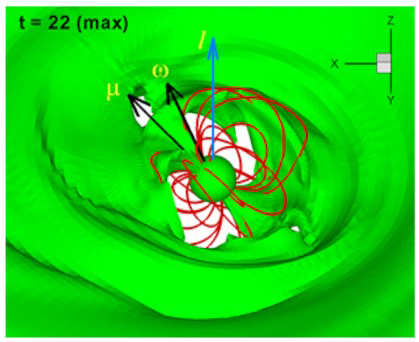
\includegraphics[width=5cm]{figs/Romanova2021fig8-panel.png}
\caption{Simulation of accretion on an inclined dipole. Mass flows towards the magnetic pole \cite{2021MNRAS.506..372R} \textcolor{blue}{need to ask for permission} \label{fig:romanova}}
\end{figure}

In one case, TW Hya, the signal is strong enough to determine the line shift of the soft X-ray lines to $38.3 \pm 5.1$~km/s \cite{2017A&A...607A..14A}. Since this is much less than the free-fall velocity, we must see the shock close perpendicular to the line-of-sight. TW~Hya is observed close to pole-on, so the accretion shocks must the located in the equatorial region.




\subsection{X-ray signatures of the accretion shock}
\label{sect:accretionobs}
{\color{blue}Moritz, Christian

Kastner & Brickhouse spectra, other spectra?, Argiroffi redshift? yes, Brickhouse 2012 variability,  naturepaper solar!, argiroffi V2129, V4046}


% Moritz list of citations to be put in the correct location later
AA Tau?

MHD modelin coal abs 2014ApJ...795L..34B 

2011A&A...526A.104C curran



The X-ray emission from cool stars on the main-sequence is caused by coronal activity. Young stars rotate faster and thus have more magnetic activity and stronger coronal X-rays than older stars such as our Sun. That is why accretion signatures are hard to find in broad-band X-ray spectra, in particular for stars embedded in a molecular cloud. To the contrary, surveys even show reduced X-ray flux correlated with accretion \cite{2005ApJS..160..401P}. However, this does not contradict the idea that accretion shocks generate soft X-rays as models show that the shock would contribute only below 1~keV \cite{1999AstL...25..430L}: Soft X-ray are frequently absorbed by circum-stellar material or the remnants of the star forming cloud, and soft X-rays from the accretion shock are not strong enough to make up for other effects that might reduce coronal activity, such as the lower rotation rate compared to disk-less stars of the same age \textcolor{blue}{reference here}.

Additional diagnostics are provided by high-resolution grating spectroscopy. Most importantly, the density of the emitting plasma can be determined from line ratios in the O~{\sc vii} and Ne~{\sc ix} triplets, which can be resolved into three lines with XMM-Newton or Chandra grating spectroscopy: A resonance line ($r$), an intercombination line ($i$), and a forbidden line ($f$). In collisionally excited plasma, the $f$ line is typically stronger than the $i$ line, but collisions in high-density plasma or strong UV fields (relevant in A or B stars, but not in the lower-mass classical T Tauri stars) can excite an electron from the upper level of the $f$ line to the upper level of the $i$ line. A low $f/i$ ratio is thus a sign of high densities in the emission region, which leads to the idea that this X-ray emission originates behind the shock front of an accretion shock. Figure~\ref{fig:softexcess} (left panel) shows examples for three CTTS which all show $f/i < 1$ compared to a typical main-sequence star with $f/i\sim 4$. This was first seen in TW~Hya \cite{Kastner_2002}, but the same pattern has since been confirmed in a number of CTTS.

\begin{figure}[t]
\centering
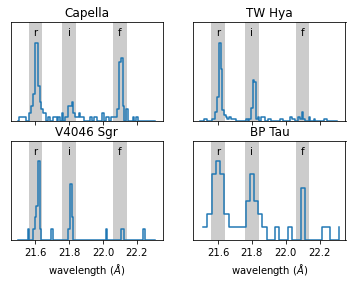
\includegraphics[width=0.49\textwidth]{figs/o7f2i.png}
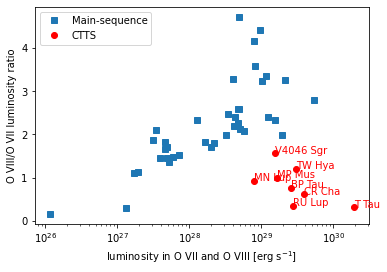
\includegraphics[width=0.49\textwidth]{figs/o72o8.png}
\caption{Signatures of accretion in classical T Tauri stars from high-resolution grating spectroscopy. \emph{Left:} Density-sensitive O~{\sc vii} triplet. Capella is a main-sequence star with an $f/i\sim 4$, while the other three sources are examples of CTTS with $f/i < 1$. All lines are unresolved, they appear wider in BP~Tau because the data is taken with a lower-resolution spectrograph (Chandra/LETG, while the other three are Chandra/HETG). \emph{Right:} Ratio of O~{\sc viii} to O~{\sc vii} line flux compared to the total flux in oxygen lines. All acrreting sources are well offset from the main-squence stars, indicating additional soft emission plasma. Modified from Ref.~ \cite{2013ApJ...771...70G} (see there for data sources) \label{fig:softexcess}}
\end{figure}

A related diagnostic is looking at the ratio of two ions of the same element. Figure~\ref{fig:softexcess} (right) shows the ratio of the flux in O~{\sc viii} to O~{\sc vii}. CTTS show lower O~{\sc viii}/O~{\sc vii} ratio than main-sequence stars of comparable luminosity, indicating CTTS emission is dominated by cooler plasma \cite{2007A&A...473..229R,2007A&A...474L..25G}. Looking from a different angle, one might also interpret this figure as  CTTS having a O~{\sc viii}/O~{\sc vii} much more in line line with low-luminosity main-sequence stars, and because there is a relation that brighter coronae are also hotter, this also leads to the conclusion that CTTS have additional cool plasma compared to normal corona. Again, this plasma can be interpreted as accretion-powered.

A third and more controversial observation is that CTTS usually show abundances that the Ne enhanced and Fe depleted compared to solar abundances. This pattern is seen in active stars, where it is attributed to element separation in the corona due to different values of the first ionization potential (FIP) of ions. Neon has a particularly high FIP and iron a particularly low one, so the pattern observed is called IFIP (inverse FIP). However, CTTS are cooler than main-sequence stars of comparable luminosity and so alternative scenarios have been discussed. Since accretion comes from the inner edge of the accretion disk, it is possible that disk process separate elements. If gain-forming elements condense into grains, pebbles, and proto-planets, the material on the inner disk edge might be depleted of Fe, Si, and similar metals, while noble gases stay in the gas phase and are thus preferentially accreted. \textcolor{blue}{HMG: This paragraph still needs some references.}

Early simulations of the accretion shock follow a 1D description of the flow. This approach is sufficient to match CCD-level resolution X-ray data. The accretion shock produces plasma matching the observed X-ray temperatures \citep{lamzin_1998} and the total energy in the accretion stream can be determined from fitting UV and optical spectra to determine the mass accretion rate \citep{calvet_1998}. Even early observations of the density-sensitive line ratios in He-like triplets such as in Fig~\ref{fig:softexcess} (left) can be explained by 1D models assuming a combination of accretion shock and coronal plasma \cite{Guenther_2007}. 

Before we discuss the shortcomings of the 1D approach and how more complex models can provide additional insight into the accretion shock structure, we want to present the fundamental physics that happens in accretion shocks. The following section assumes 1D for simplicity.


\subsection{Physics of accretion in 1D}
\label{sect:accretionphysics}

Accretion happens when mass from the circumstellar disk is transferred onto the stellar surface. In the basic model of magnetically funneled accretion, the stellar high-energy radiation ionizes the inner edge of the disk. When the stellar magnetic field connects to the inner edge of the disk, matter can flow along the field lines and impact onto the star, where a strong shock forms. The accretion column is relatively cool, but in the shock that gas is heated up to X-ray emitting temperatures. Depending on the exact location of the shock, those X-rays may or may not be visible, but the shock certainly heats the surrounding photosphere, which causes bright UV emission and an optical veiling (a strong continuum that makes phtotospheric emission lines appear weaker than in a non-accretion star.)

As the star and the disk rotate, and the magnetic field and the disk structure evolves, the accretion geometry and the accretion rate can change on time scales as short as minutes or as long as centuries; accretion can also switch off temporarily or permanently, as the star looses its disk. Despite that, many basic aspects of the accretion physics can be described in a 1D model where all mass motion happens parallel to the magnetic field. In the next few sub-sections we review some of the basic physics of accretion columns and accretion shocks. While modern models go far beyond such a simple prescription, the foundation of all accretion shock models still is to convert the graviational energy in the disk to kinetic energy of the infalling gas, which in turn gets turned into heat and radiation in the accretion shock.

\subsubsection{Free-fall velocity}
The free fall velocity $v_{\textnormal{free}}$ of material coming from an inner disk radius of $R_\mathrm{in}$ onto a star with mass $M_*$ and radius $R_*$ is
\begin{equation} 
v_{\textnormal{free}} = \sqrt{{2GM_*} \left(\frac{1}{R_*} - \frac{1}{R_\mathrm{in}}\right)} \approx 620 \sqrt{\frac{M_*}{M_\odot}}\sqrt{\frac{R_\odot}{R_*}} \frac{\textnormal{km}}{\textnormal{s}}\ \label{eqn:freefall} 
\end{equation}
where $G$ is the gravitational constant. The inner radius is typically a few stellar radii and thus $v_\textnormal{ff}$ is very close to infall from infinity.


\subsection{Calculation of shock front}
All turbulent fluxes are neglected and we only treat stationary shocks. In the shock front, ions and electrons are heated differently, but they remain strongly coupled and reach the same temperatures with in a few mean-free path lengths - a region so thin that it is justified to treat them as a single fluid. 

Somewhere along the accretion column, a shock forms when the forward ram pressure becomes comparable to the pressure of the underlying material. The shock front itself is very thin, only of the order of a few mean free paths \cite{raizerzeldovich}. Therefore it can be treated as a mathematical discontinuity described by the Rankine-Hugoniot jump-conditions \cite[][chap.~7, \S~15]{raizerzeldovich}; in the shock the super-sonic infall velocity is converted mostly into thermal energy. To simplify the numerical treatment we assume the direction of flow parallel to the magnetic field, so the Lorentz force does not influence the dynamics. Marking the state in front of the shock front by the index 0, that behind the shock by index 1, the Rankine-Hugoniot conditions become
\begin{eqnarray}
\rho_0 v_0 &=& \rho_1 v_1 \label{RH1}\\
P_0+\rho_0 v_0^2 &=& P_1+\rho_1 v_1^2 \label{RH2}\\
\frac{5 P_0}{2\rho_0}+\frac{v_0^2}{2}&=&\frac{5 P_1}{2\rho_1}+\frac{v_1^2}{2} \ ,\label{RH3}
\end{eqnarray}
where $v$ is the velocity, $\rho$ the total mass density of the gas and $P$ its pressure. 

From the jump conditions, the shocks will heat gas to a temperature
\begin{equation}
kT \simeq \frac{3}{16}\mu m_p v^{2} \approx 0.3\,{\rm keV}\left(\frac{v}{500\,{\rm km/s}}\right)^{2} \approx3.5\times10^6\,{\rm K} \left(\frac{v}{500\,{\rm km/s}}\right)^{2},
\label{eqn:Tshock}
\end{equation}
where $\mu$ is the dimensionless atomic weight.

\subsubsection{Structure of the post-shock region}

In the following section we compute how the originally different kinetic temperatures of ions and electrons as well as the ionisation temperature
equilibrate and calculate the emitted X-ray spectrum.

\paragraph{Momentum balance}\label{hydrodyn}

In the post-shock region the gas emits radiation and cools down, so the energy of the gas is no longer conserved.  However, the particle number flux $j$ of ions (and atoms) 
\begin{equation}j=nv\label{j_n}\end{equation}
is conserved, where $n$ is the ion/atom number density; the electron number density is denoted by $n_{\mathrm{e}}$. The total momentum flux $j_p$ is conserved, since we ignore the momentum loss by radiation; it consists of the ion and the electron momentum as follows:
\begin{eqnarray}  
j_p&=&\mu m_{\mathrm{H}} n v^2+P \nonumber \\
   &=&\mu m_{\mathrm{H}} n v^2+nkT \label{j_p}
\end{eqnarray}
with $P$ is the thermodynamic pressure and $T$ the temperature; $m_{\mathrm{H}}$ denotes the mass of a hydrogen atom.

\paragraph{Energy balance}
\label{sect:energybalance}

Let us next consider the energy balance in the post-shock region. In general,  
\begin{equation} \label{tsminuspdvisdu} T d\Sigma -P dV=dU \end{equation}
where $\Sigma$ denotes the entropy and $U$ the internal energy of the plasma. The quantity $T d\Sigma=dQ$ denotes the heat flux through the boundaries of the system; one important component of the is the energy loss $Q_{col}$ through collisions that excite higher electronic states, which will than decay through radiation. 

Assuming that the shock location is stationary, we get $\frac{d}{dt}=\frac{\partial}{\partial t}+\frac{\partial z}{\partial t}\frac{\partial}{\partial z}=v\frac{\partial}{\partial z}$ depending on the location $z$, measured from the shock front inwards; differentiation with respect to $z$ will be indicated by $'$.
The internal energy $U$ is in this case the thermal energy $U=\frac{3}{2}kT$, the pressure $P$ can be rewritten using the equation of state. The specific volume $V$ is the inverse of the number density $V=\frac{1}{n}$. 
It is convenient to write the electron number density as \mbox{$n_{\mathrm{e}}=x_e n$,} with $x_e$ denoting the number of electrons per heavy particle.
\begin{equation}
\label{energyelec}
v\left(\frac{3}{2}x_e k T_{\mathrm{e}}\right)'+v x_e n k T_{\mathrm{e}} \left(\frac{1}{n}\right)'=-Q_{col} x_e n,
\end{equation} 

We now have $n$, $v$, and $T$ as variables and three hydrodynamic equations (\ref{j_n}, \ref{j_p}, and \ref{energyelec}), so the structure of the post-shock region can be calculated.


\subsection{Observed shortcomings of stationary 1D models}
While 1D models are successful in many aspects, there are observational and theoretical arguments that important physical processes are not captured in 1D. In deep Chandra observations of TW~Hya, densities can be measured in three density-sensitive triplets. The density is highest in Mg~{\sc xi} and lowest in O~{\sc vii}, although Mg~{\sc xi} is formed at a higher temperature \cite{Brickhouse_2010}. Thus, one would expect Mg~{\sc xi} emission from a region directly behind the accretion shock and O~{\sc vii} from denser layers deeper down. One possible explanation is that the observed O~{\sc vii} emission is not from the accretion shock itself, but originates in hot material that escapes the accretion column to the side and is denser than a normal stellar corona, but not as dense as plasma behind the accretion shock. That in turn means that the total X-ray flux might not be a good measure of the total accretion rate. 

This is corroborated by the surprising observation that X-ray determined mass accretion rates are very similar for most sources despite a difference in optically determined mass accretion rate by three orders of magnitude \cite{2011A&A...526A.104C} which can be explained if the accretion streams are not homogeneous structures but have a density profile and the inner layers either form shocks deeper in the atmosphere or simply have they X-ray emission reprocessed by the outer layers of the accretion stream \cite{2018A&A...618A..55S,2021Natur.597...41E}.

Time variability can give us another insight. In V4046~Sgr the emission lines from soft, presumably shocked, plasma have a period of exactly have the orbital period of the close binary. Together with Doppler-imaging this leads to the interpretation that we can observe the shock only when the accretion flow is perpendicular to the line of sight, while the accretion funnel blocks the view of the shocked region at other times \cite{2012ApJ...752..100A}. Similarly, the accretion funnel has been observed to block the X-rays from AA~Tau for certain rotational phases. This includes coronal and accretion generated X-rays \cite{2007A&A...462L..41S,2007A&A...475..607G}. 
There are several other classes of time-variable pre-main sequence accretors, including FU~Ors and EX~Ors, where the accretion rate changes by orders of magnitude or stars where a change in the disk structure moves absorbing material into our light of sight, such as in RW~Aur or also in AA~Tau. However, those changes happen on much larger scales than the accretion shock itself and are not discussed here any further.

Similarly, improved models including LTE radiation transfer now show that the heated photosphere does not radiate as a simple black body in the optical and infrared \cite{Dodin_2012,Dodin_2013}, but that is also produces lines, which selectively fill in some photospheric absorption lines, possibly biasing accretion rate measurements based on optical veiling.



\begin{figure}
    \centering
    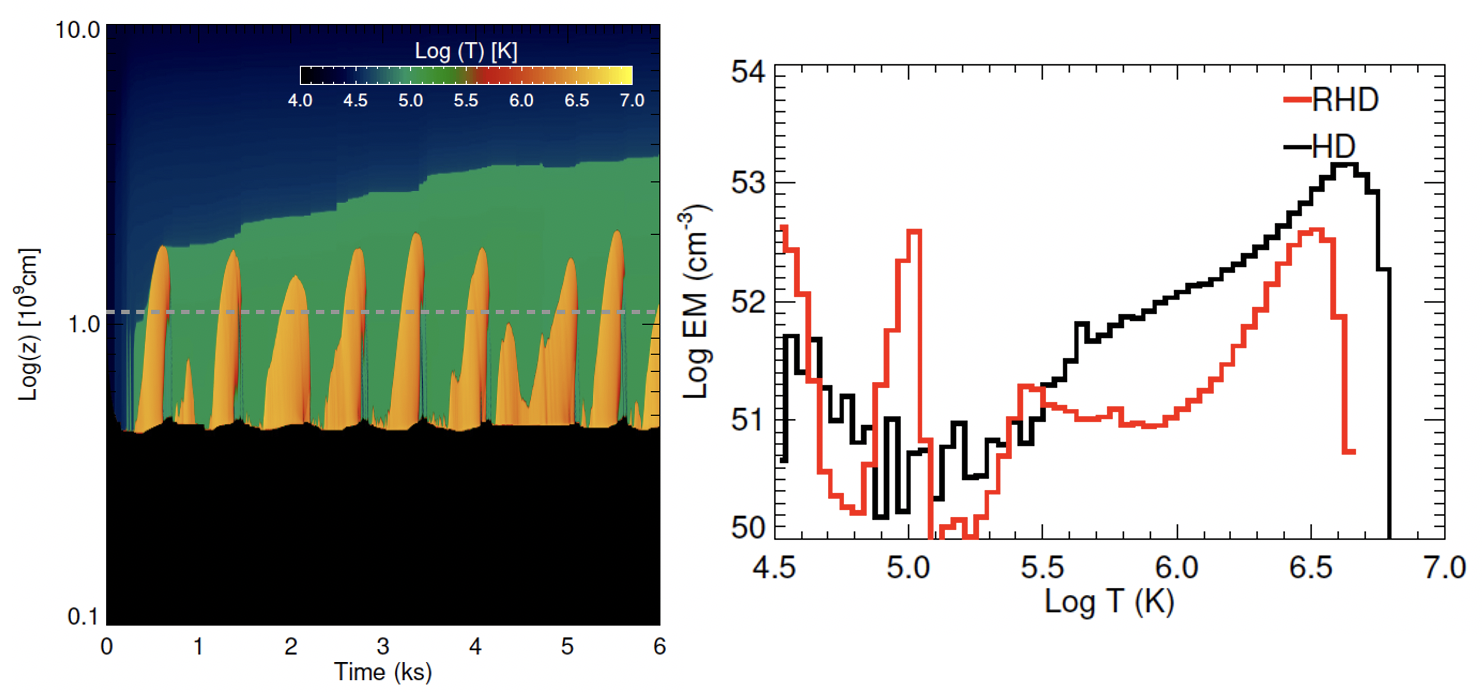
\includegraphics[width=11cm]{figs/colombo2019b.png}
    \caption{A combination of Fig. 3 and Fig. 5 from Colombo et al. 2019b. As far as I know the only non-LTE simulation of the accretion region. Need from permission. I would select one of the figures, Colombo 2016 or Colombo 2019b.}
    \label{fig:colombo2016}
\end{figure}

\begin{figure}
    \centering
    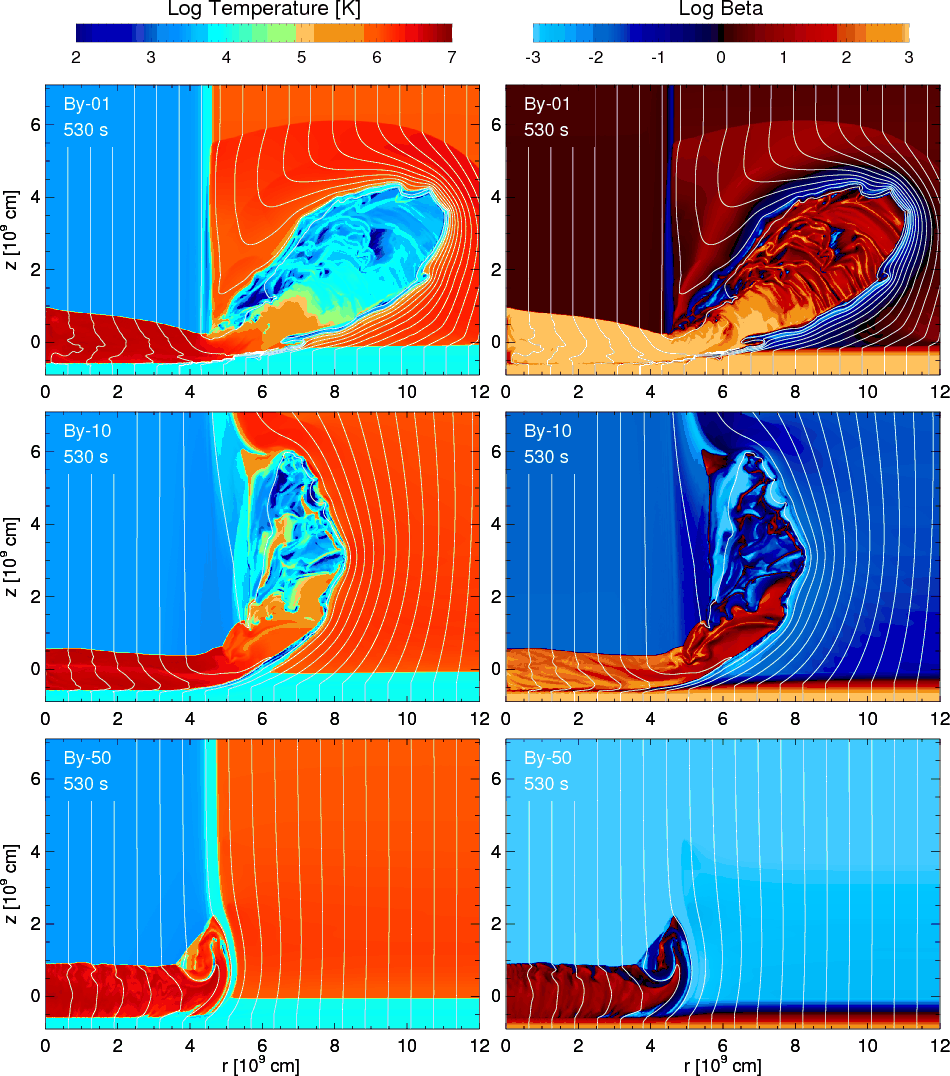
\includegraphics[width=11cm]{figs/Sacco2010.png}
    \caption{Moritz: I've always liked this figure. It's over a decade old at this point but it has the "spill-out" on the side that observers often have in mind and I think it's easier to interpret than a figure with time on the x-axis. Or is this so out of date that it's simply not OK to use that any longer? THe REvet et al 2017 would work for the same purpose. I would select one of the figures, Colombo 2016 or Colombo 2019b or this one.}
    \label{fig:sacco2016}
\end{figure}

\textcolor{blue}{
- When we start to talk about numerical models we should introduce MHD equations. Transition from analytical to numerical models in this subsection?}

\textcolor{blue}{- I would not call the models above this section "analytical". Lamzin 2004, Calvet \& Gulbring and my own Guenther 2007 are all numerical models solving HD equations - admittedly in 1D, but including radiative losses, so it's a numerical, not an analytic solution. So, in my mind, the questions is if we transition from 1D HD (some of those models might be 1D MHD, but if the B field is parallel to the one model dimension you have, that's essentially HD) to 3D MHD and this might be a good place to do that.}

\subsection{The multi-D structure of the accretion shock}

Most observations of the structure of the accretion shock on young stars are spatially unresolved; only Doppler-imaging can at least reveal the location on the surface where the accretion shock happen. Yet, it would be very valuable to learn about the detailed 3D geometry and the time evolution of accretion shocks to interpret the unresolved data. For example, it is unclear if the accretion shocks forms deeply in the photosphere where it is hidden from view or higher up in the accretion funnel. One approach to address this problem is to perform experiments in the laboratory using a set-up where magnetic fields, densities, temperatures, and other hydrodynamical parameters are chosen to scale to the stellar case. Such work finds that plasma is ejected laterally from the accretion shock and forms a shell around the infalling stream \cite{2017SciA....3E0982R} . This hot shell provides an additional absorber that reduces the shock emission that is directly observable. Recently, new laboratory experiments tested accretion streams not perpendicular to the impacted surface as it might happen for accretion stream along complex magnetic field structures. They find the resulting plasma flows to be highly asymmetric and see a large amount of plasma escaping laterally from the accretion flow \cite{2020A&A...642A..38B}.  

Another approach is to look for analogous situations in our Sun, where spatially resolved data in the UV and EUV, even if not in X-rays, is available with long time coverage and high cadence. One particular event happened on June, 7$^{th}$, 2011, when parts of an erupting filament fell back into the Sun \cite{2013Sci...341..251R,2013A&A...559A.127O}. The infall speed of up to 450~km/s was comparable to free-fall accretion onto T Tauri stars, but the accretion rate was obviously much lower. Similar to the laboratory experiments, the initial infall triggered upflows, but here they shocked with later fragments causing UV emission.

Both, laboratory experiments and the solar analogy, point to a significantly more complex picture than the simple 1D accretion shock outlined above. Simulations of the accretion shock \textcolor{blue}{Sabrina, do you want to conitnue here? Structure of the accretion shock in X-rays: Orlando, Bonito, Colombo; figure?}

\begin{figure}
    \centering
    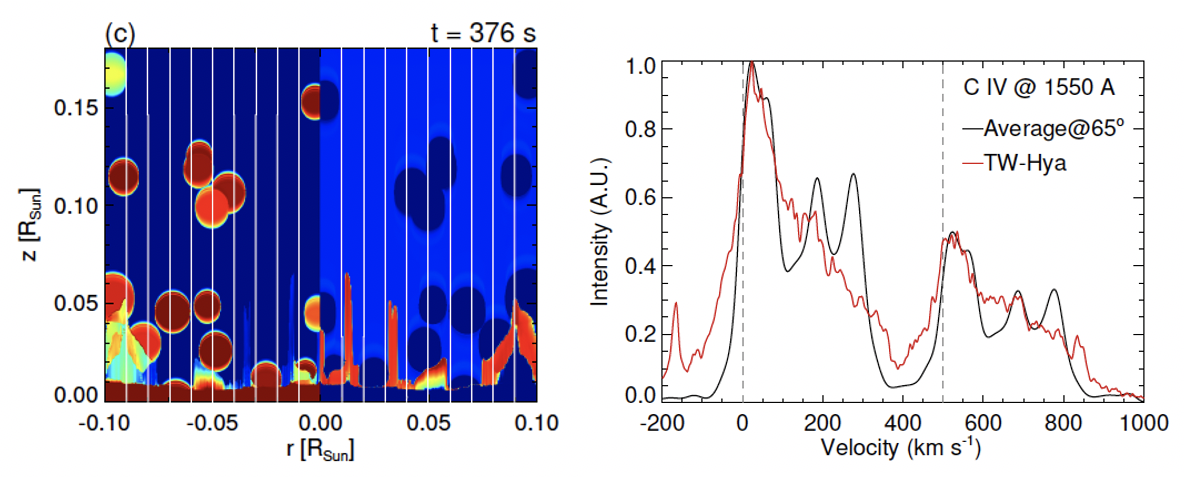
\includegraphics[width=11cm]{figs/colombo2016.png}
    \caption{A combination of Fig. 3 and Fig. 6 from Colombo et al. 2016. Interesting for the fragmented structure of the accretion stream which reproduces the CIV profiles (X-rays and other observations). Need for permission. I would select one of the figures, Colombo 2016 or Colombo 2019b.}
    \label{fig:colombo2016}
\end{figure}

\begin{figure}
    \centering
    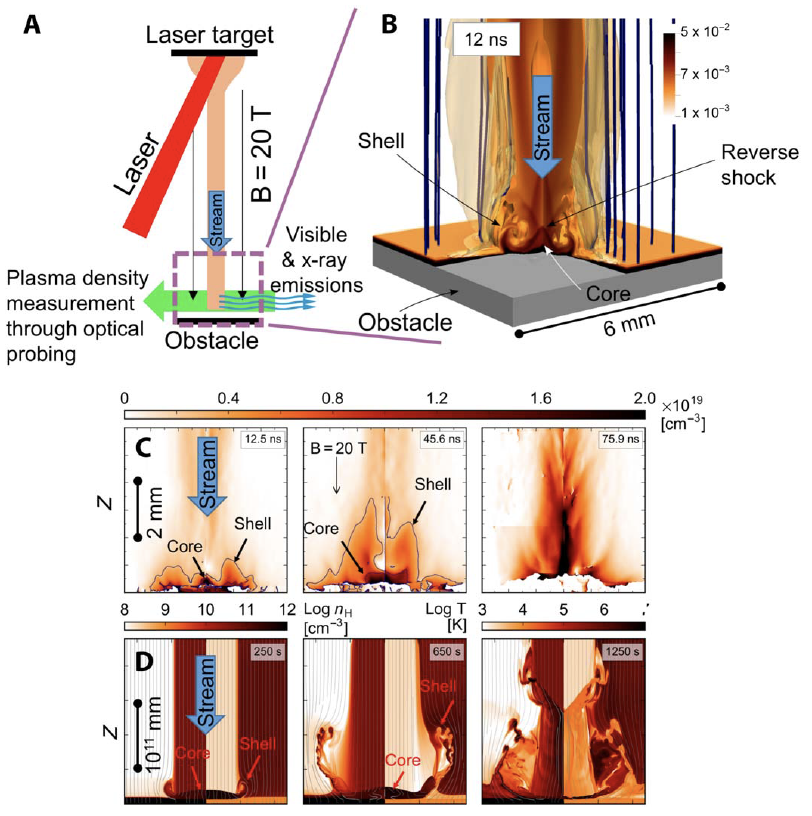
\includegraphics[width=11cm]{figs/Revet2017.png}
    \caption{Another possibility from Revet et al. 2017. Here they combine laboratory experiments with MHD simulations. Need to ask for permission.}
    \label{fig:revet2017}
\end{figure}
